We describe how to use causality for a given DyNetKAT expression.

\begin{definition}
    Given sets of events $E_0$ and $E_1$ let
    $E = \s{(0,e)|e \in E_0} \cup \s{(1,e)|e \in E_1}$.
    We define injections $\iota_k: E_k \rightarrow E$, given by
    $\iota_k(e) = (k,e)$, for $k = 0,1$.
\end{definition}

\begin{definition}
    Given sets of events $E_0$ and $E_1$ let their product $E$ be:
    \begin{align*}
        E_0 \times_* E_1 = \s{(e_0,*)|e_0 \in E_0} \cup \s{(e_0,*)|e_0 \in E_0}
        \cup \s{(e_0,e_1)|e_0 \in E_0 \wedge e_1 \in E_1}
    \end{align*}
    We define projections $\pi_i: E \rightarrow_* E_i$, given by
    $\pi_i(e_0,e_1) = e_i$, for $i=0,1$.
\end{definition}

\begin{definition}
    Let $\mathrm{E} = (E,\#,\vdash,L,l)$ be a labeled event structure and
    $M = \mathfrak{M}(\mathrm{E})$ be its causal model.
    Let $\alpha$ be a label and $\mathrm{E'} = \alpha \mathrm{E}$.
    We define $M' = \alpha M$ to be a causal model where:
    \begin{align*}
        \mathcal{V'} = & \s{C'_{e_i,e_j} |  1 \leq i < j \leq n.
        e_i \in E' \amp e_j \in E'}                                 \\
                       & \cup \s{EN'_{s,e} | s \in \mathcal{P}(E'),
        e \in E'. e \not \in s }                                    \\
                       & \cup \mathcal{V}
    \end{align*}
    Next, we define functions of $M'$ as follows:
    $$
        \f{C'_{e,e'}} = \begin{cases}
            \T       & \text{ if } e = (0,\alpha) \vee e' = (0,\alpha) \\
            C_{e,e'} & \text{ otherwise }
        \end{cases}
    $$

    $$
        \f{EN'_{s,e}} = \begin{cases}
            \T                      & \text{ if } e = (0,\alpha)             \\
            EN_{s',e} \wedge Con(s) & \text{ if } s = s' \cup \s{(0,\alpha)} \\
            \F                      & \text{ otherwise }
        \end{cases}
    $$
\end{definition}

\begin{definition}
    Let $\mathrm{E}_0 = (E_0,\#_0,\vdash_0,L_0,l_0)$ and
    $\mathrm{E}_1 = (E_1,\#_1,\vdash_1,L_1,l_1)$ be labeled event structures
    and $M_0,M_1$ be their causal models.
    Let $(E',\#',\vdash',L',l') = \mathrm{E_0} + \mathrm{E_1}$.
    We define $M' = M_0 + M_1$ to be a causal model where we have:
    \begin{align*}
        \mathcal{V} = & \s{C_{e_i,e_j} |  1 \leq i < j \leq n.
        e_i \in E' \amp e_j \in E'}                               \\
                      & \cup \s{EN_{s,e} | s \in \mathcal{P}(E'),
        e \in E'. e \not \in s }                                  \\
                      & \cup \mathcal{V}_0 \cup \mathcal{V}_1
    \end{align*}
    We define the functions of $M'$ as follows:
    $$
        \f{C_{e,e'}} = \begin{cases}
            \T         & \text{ if } \exists e_0,e_1.
            (e = \iota_0(e_0) \wedge e' = \iota_1(e_1))
            \vee (e' = \iota_0(e_0) \wedge e = \iota_1(e_1))            \\
            C^0_{e,e'} & \text{ if } \exists e_0,e_0'. e = \iota_0(e_0)
            \wedge e' = \iota_0(e_0')                                   \\
            C^1_{e,e'} & \text{ if } \exists e_1,e_1'. e = \iota_1(e_1)
            \wedge e' = \iota_1(e_1')
        \end{cases}
    $$
    $$
        \f{EN_{s,e}} = \begin{cases}
            Con(s) \wedge EN^0_{s_0,e_0} & \text{ if }
            \exists s_0 \in Con_0,e_0 \in E_0. s = \iota_0(s_0) \\
            Con(s) \wedge EN^1_{s_1,e_1} & \text{ if }
            \exists s_1 \in Con_1,e_1 \in E_1. s = \iota_1(s_1) \\
            \F                           & \text{ otherwise }
        \end{cases}
    $$
\end{definition}

\begin{definition}
    Let $\mathrm{E}_0 = (E_0,\#_0,\vdash_0,L_0,l_0)$ and
    $\mathrm{E}_1 = (E_1,\#_1,\vdash_1,L_1,l_1)$ be event structures and
    $M_0,M_1$ be their causal models.
    Let $(E',\#',\vdash',L',l') = E_0 \times E_1$.
    We define $M' = M_0 \times M_1$ to be a causal model where we have:
    \begin{align*}
        \mathcal{V} = & \s{C_{e_i,e_j} |  1 \leq i < j \leq n.
        e_i \in E' \amp e_j \in E'}                               \\
                      & \cup \s{EN_{s,e} | s \in \mathcal{P}(E'),
        e \in E'. e \not \in s }                                  \\
                      & \cup \mathcal{V}_0 \cup \mathcal{V}_1
    \end{align*}
    We define the functions of $M'$ as follows:
    $$
        \f{C_{e,e'}} = \begin{cases}
            \T & \text{ if } \pi_0(e) = \pi_0(e') \vee \pi_1(e) = \pi_1(e') \\
            C^0(\pi_0(e),\pi_0(e')) \vee  C^1(\pi_1(e),\pi_1(e'))
               & \text { if } \pi_0(e) \neq * \wedge \pi_1(e) \neq *        \\
            C^0(\pi_0(e),\pi_0(e'))
               & \text { if } \pi_1(e) = *                                  \\
            C^1(\pi_1(e),\pi_1(e'))
               & \text { if } \pi_0(e) = *                                  \\
        \end{cases}
    $$
    $$
        \f{EN_{s,e}} = \begin{cases}
            EN^0(\pi_0(s),\pi_0(e)) \wedge EN^1(\pi_1(s),\pi_1(e))
                                    & \text{ if } \pi_0(e) \neq * \wedge \pi_1(e) \neq * \\
            EN^0(\pi_0(s),\pi_0(e)) & \text{ if } \pi_1(e) = *                           \\
            EN^1(\pi_1(s),\pi_1(e)) & \text{ if } \pi_0(e) = *                           \\
        \end{cases}
    $$
\end{definition}
\begin{definition}
    Let $\mathrm{E} = (E,\#,\vdash,L,l)$ be an event structure and $M$ its
    causal model.
    For each variable $v \in \mathcal{V}$ we define a function $l(v)$ which
    returns the set of labels of this variable regarding the $l$ as follows:
    $$
        l(v) = \begin{cases}
            \s{l(e),l(e')}                     & \text{ if } \exists e,e' \in E. v = C_{e,e'} \\
            \s{l(e')| e' \in s } \cup \s{l(e)} & \text{ if }
            \exists s \subseteq E, e \in E. v = EN_{s,e}
        \end{cases}
    $$
\end{definition}

\begin{definition}
    Let $\mathrm{E} = (E,\#,\vdash,L,l)$ be an event structure and $M$ its
    causal model.
    Given a set of labels $\Lambda$, we define $M' = M\lceil \Lambda$ to be
    a causal model where we have removed any variable such as
    $x \in \mathcal{V}$ and its functions where $l(v) \not \subseteq \Lambda$.
\end{definition}

\begin{example}
    Consider the following network where we want to check a blacklist
    property, i.e. no packets arrive at $d$:
    \begin{center}
        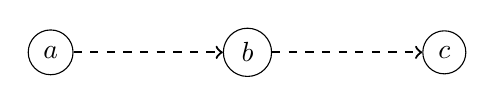
\begin{tikzpicture}[node distance={25mm},
                main/.style = {draw, circle},
                d/.style = {->,thick,dashed} ]
            \node[main] (a) {$a$};
            \node[main] (b) [right of=a] {$b$};
            \node[main] (c) [right of=b] {$c$};
            \draw[d] (a) -- (b);
            \draw[d] (b) -- (c);
        \end{tikzpicture}
    \end{center}
    We define this network using the following DyNetKAT term:
    \begin{align*}
        S_{xy}  & = l = x \cdot l \la y              \\
        P       & = u!S_{ab}                         \\
        Q       & = u!S_{bc}                         \\
        N_{x,y} & = (S_x+S_y)^* \oplus u?x';N_{x',y}
        \oplus u?y';N_{x,y'}                         \\
        SDN     & = N_{0,0} \parallel P \parallel Q
    \end{align*}
    We may rewrite the terms as follows:
    \begin{align*}
        N_{0,0}   & = u?S_{ab};N_{ab,0} \oplus u?S_{bc};N_{0,bc} \\
        N_{ab,0}  & = S_{ab}^* \oplus u?S_{bc};N_{ab,bc}         \\
        N_{0,bc}  & = S_{bc}^* \oplus u?S_{ab};N_{ab,cd}         \\
        N_{ab,bc} & = (S_{ab}+S_{bc})^*
    \end{align*}
    Given a packet $\sigma$ where $\sigma(l) = a$ we can replace NetKAT
    policies with actions of the form $(\sigma, \sigma')$.
    In this network we denote the action $(\sigma, \sigma')$
    with $xy$ where $\sigma(l) = x$ and $\sigma'(l) = y$.
    Let $N'_{x,y}$ be the term where we replaced NetKAT policies with
    actions of the form $(\sigma,\sigma')$ and let we use $p,p',q,q'$ to
    denote the actions $u?S_{ab},u!S_{ab},u?S_{bc},u!S_{bc}$.
    We also restrict the network by forbidding actions in 
    $\mathcal{L}=\s{p,p',q,q'}$.
    Thus we have:
    \begin{align*}
        SDN'       & = \delta_{\mathcal{L}}(N'_{0,0} \parallel P \parallel Q) \\
        P'         & = p'                                                     \\
        Q'         & = q'                                                     \\
        N'_{0,0}   & = p;N'_{ab,0} \oplus q;N'_{0,bc}                         \\
        N'_{ab,0}  & = ab \oplus q;N'_{ab,bc}                                 \\
        N'_{0,bc}  & = p;N'_{ab,bc}                                           \\
        N'_{ab,bc} & = ab \oplus ac
    \end{align*}
    \begin{center}
        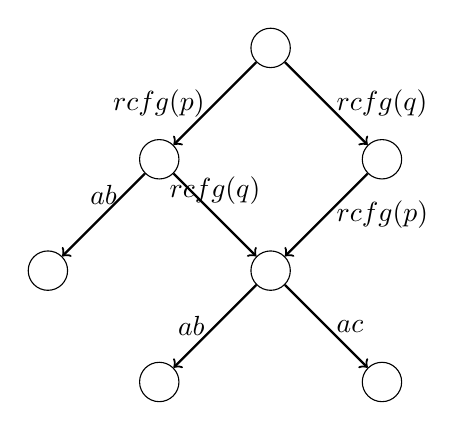
\begin{tikzpicture}[node distance={20mm},
                main/.style = {draw, circle,minimum width=5mm},
                s/.style = {->,thick}]
            \node[main] (s1) {};
            \node[main] (s2) [below left of=s1] {};
            \node[main] (s3) [below right of=s1] {};
            \node[main] (s4) [below left of=s2] {};
            \node[main] (s5) [below right of=s2] {};
            \node[main] (s6) [below left of=s5] {};
            \node[main] (s7) [below right of=s5] {};
            \draw[s] (s1) -- node[left]{$rcfg(p)$} (s2);
            \draw[s] (s1) -- node[right]{$rcfg(q)$}(s3);
            \draw[s] (s2) -- node[above]{$ab$}(s4);
            \draw[s] (s2) -- node[above]{$rcfg(q)$}(s5);
            \draw[s] (s3) -- node[right]{$rcfg(p)$}(s5);
            \draw[s] (s5) -- node[left]{$ab$}(s6);
            \draw[s] (s5) -- node[right]{$ac$}(s7);
        \end{tikzpicture}
    \end{center}
\end{example}